\section{Implementation}
\label{sec:implementation}

% source langauge
OpenRAM's methodology is implemented using an object-oriented approach
in the Python programming language. Python is a simple, yet powerful
language that is easy to learn and very human-readable. Moreover, Python
enables portability to most operating systems. OpenRAM has no additional
dependencies except a DRC/LVS tool, but that is disabled with a
warning if the tools are unavailable.

% portability of tools and technologies
In addition to system portability, OpenRAM is also translatable across
numerous process technologies. This is accomplished by using
generalized routines to generate the memory based on common features
across all technologies. To facilitate user modification and
technology interoperability, OpenRAM provides a reference implementation in
$45$nm FreePDK45~\cite{4231502} and a fabricable option using the
MOSIS Scalable CMOS (SCMOS) design rules~\cite{scmos}. FreePDK45 uses
many design rules found in modern technologies, but is non-fabricable,
while SCMOS enables fabrication of designs using the MOSIS foundry
services. SCMOS is not confidential and an implementation using it is
included, however, it does not include many advanced DSM design
rules. OpenRAM has also been ported to other commercial technologies,
but these are not directly included due to licensing issues.

% methodology overview
OpenRAM's framework is divided into \enquote{front-end} and \enquote{back-end}
methodologies as shown in Figure~\ref{fig:methodology}. The front-end
has the compiler and the characterizer. The compiler generates
SPICE models and its GDSII layouts based on user inputs. The
characterizer calls a SPICE simulator to produce timing and power
results. The back-end uses a spice netlist extracted from the GDSII
layout using to generate annotated timing and power models.

\begin{figure}[tb]
\centering
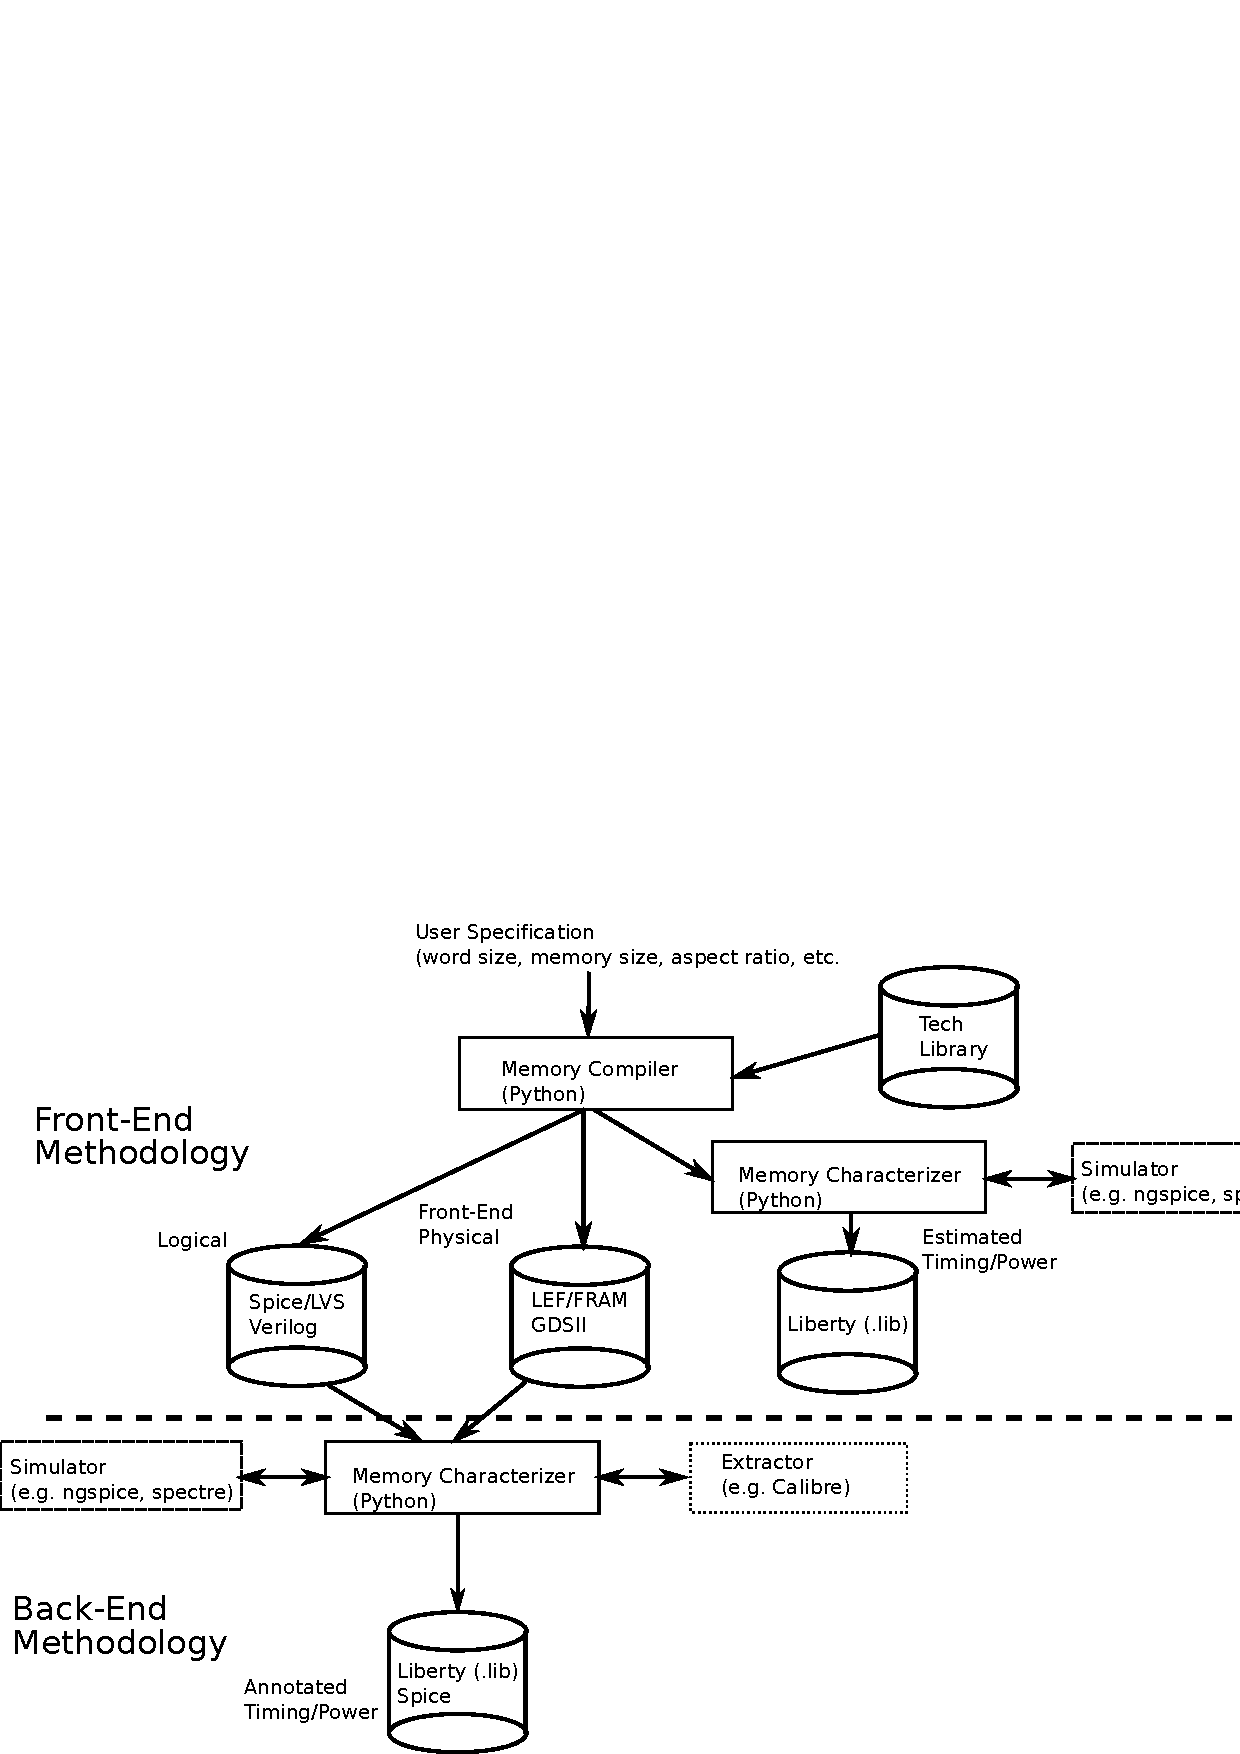
\includegraphics[width=8cm]{./figs/methodology.pdf}
\caption{Overall Compilation and Characterization Methodology}
\label{fig:methodology}
\end{figure}

%\fixme{We actually dont have back end done yet.}

\subsection{Base Data Structures}

The design modules in OpenRAM are derived from the {\it design} class
(design.py). The design class has a name, a SPICE model (netlist), and
a layout. Both the SPICE model and the layout inherit their
capabilities from a hierarchical class. The design class also provides
inherited functions to perform DRC and LVS verification of any
sub-design for hierarchical debugging.

The design class derives from the {\it spice} class
(hierarchy\_\allowbreak spice.py) which has a data structure to
maintain the circuit hierarchy. This class maintains the design
instances, their pins, and their connections as well as helper
functions to maintain the structure and connectivity of the circuit
hierarchy.

The design class also derives from a {\it layout} class (hierarchy\_layout.py).
This class has a list of physical instances of sub-modules in the layout and
a structure for simple objects such as shapes and labels in the
current hierarchy level. In addition, there are helper functions that
maintain the physical layout structures.

OpenRAM has an integrated, custom GDSII library to read, write, and
manipulate GDSII files. The library, originally called
GdsMill~\cite{gdsmill}, has been modified, debugged, and extended for
OpenRAM. Full rights were given to include the GdsMill source with
OpenRAM, but to make the interfacing easier and porting to other
physical layout databases possible, OpenRAM implements a {\it
  geometry} wrapper class (geometry.py) that abstracts the GdsMill
library.

\subsection{Technology and Tool Portability}

% technology overview
OpenRAM is technology-independent by using a technology directory that
includes the technology's specific information, rules, and library
cells. Technology parameters such as the design rule check (DRC) rules
and the GDS layer map are required to ensure that the dynamically
generated designs are DRC clean. Custom designed library cells such as
the memory cell and the sense amplifier are also placed in this
directory. A very simple design rule parameter file has the most
important design rules for constructing basic interconnect and
transistor devices. FreePDK45 and SCMOS reference technologies are provided.

% hand-optimized cells
OpenRAM uses some custom-designed library primitives as technology
input. Since density is extremely important, the following cells are
pre-designed in each technology: 6T cell, sense amplifier,
master-slave flip-flop, tri-state gate, and write driver. All other
cells are generated on-the-fly using parameterizable transistor and
gate primitives.

% technology specific features
OpenRAM can be used for various technologies since it creates the
basic components of memory designs that are common over these
technologies. For technologies that have specific design requirements,
such as specialized well contacts, the user can include call-back
helper functions in the technology directory. This is done so that the
main compiler remains free of dependencies to specific technologies.

% DRC and LVS
OpenRAM has two functions that provide a wrapper interface with DRC
and LVS tools. These two functions perform DRC and LVS using the GDSII
layout and SPICE netlist files. Since each DRC and LVS tool has
different output, this routine is customized per tool to parse DRC/LVS
reports and return the number of errors while also outputting debug
information. These routines allow flexibility of any DRC/LVS tool,
but the default implementation calls Calibre nmDRC and nmLVS. In
OpenRAM, both DRC and LVS are performed at all levels of the design
hierarchy to enhance bug tracking. DRC and LVS can be disabled for
improved run-time or if tool licenses are not available.

\subsection{Class Hierarchy}

\subsubsection{High-Level Classes}

The {\it openram} class (openram.py) organizes execution and
instantiates a single memory design using the {\it sram} class. It
accepts user-provided parameters to generate the design, performs the
optional extraction, performs characterization, and saves the
resulting design files.

The {\it sram} class (sram.py) decides the appropriate internal parameter
dependencies shown in Table~\ref{table:variables}. They are dependent 
on the user-desired data word size, number of words, and number of banks.
It is responsible for instantiation of the single control logic module which
controls the SRAM banks. The control logic ensures that only one bank
is active in a given address range.

The {\it bank} class (bank.py) does the bulk of the non-control memory layout. It
instantiates $1$, $2$, or $4$ bit-cell arrays and coordinates the row and column
address decoders along with their pre-charge, sense amplifiers, and input/output
data flops.

\begin{table}
\centering
\caption{Dependencies required for sub-modules}
\begin{tabular}{|c|l|} \hline
Variable&Equation \\ \hline
\texttt{Total Bits} & $word\_size*num\_words$ \\ \hline
\texttt{Words Per Row} & $\sqrt(num\_words)/word\_size$ \\ \hline
\texttt{Num of Rows} & $num\_words/words\_per\_row$ \\ \hline
\texttt{Num of Cols} & $words\_per\_row*word\_size$ \\ \hline
\texttt{Col Addr Size} & $\log_2(words\_per\_row)$ \\ \hline
\texttt{Row Addr Size} & $\log_2(num\_of\_rows)$ \\ \hline
\texttt{Total Addr Size} & $row\_addr\_size + col\_addr\_size$ \\ \hline
\texttt{Data Size} & $word\_size$ \\ \hline
\texttt{Num of Bank} & $num\_banks$ \\ \hline
\end{tabular}
\label{table:variables}
\end{table}

\subsubsection{Block Classes}

Every other block in the memory design has a class for its base cell
(e.g., sense\_amplifier.py) and an array class (e.g.,
sense\_amplifier\_array.py) that is responsible for tiling the base
cell. Each class is responsible for physically placing and logically
connecting its own sub-circuits while passing its dimensions and port
locations up to higher-level modules.

\subsubsection{Low-Level Classes}

OpenRAM provides parameterized transistor and logic gate
classes that help with technology portability. These classes generate
a technology-specific transistor and simple logic gate layouts so that
many modules do not rely on library cells. It is also used
when a module such as the write driver needs transistor sizing
to optimize performance. The parameterized transistor (ptx.py) generates a
basic transistor of specified type and size. The parameterized
transistor class is used to provide several parameterized gates
including pinv.py, nand2.py, nand3.py, and nor2.py.

% FIXME
% crude fix to preven widow Section
%\clearpage
\subsection{Characterization}

% overview
OpenRAM includes a memory characterizer that measures the timing and
power characteristics through SPICE simulation. The
characterizer has four main stages: generating the SPICE stimulus,
running the circuit simulations, parsing the simulator's output, and
producing the characteristics in a Liberty (.lib) file. 

% standard format of stimulus
The stimulus is written in standard SPICE format and can be used with
any simulator that supports this. The stimulus only uses the
interface of the memory (e.g., bi-directional data bus, address bus,
and control signals) to perform \enquote{black box} timing measurements.

% what is measured and how
Results from simulations are used to produce the average power,
setup/hold times, and timing delay of the memory design. Setup and
hold times are obtained by analyzing the flip-flop library cell
because OpenRAM uses a completely synchronous input interface. The
setup time, hold time, and delay are found using a fast bisection
search.

\subsection{Unit Tests}

Probably the most important feature of OpenRAM is the set of thorough
regression tests implemented with the Python unit test framework.
These unit tests allow users to add features and easily verifying if
functionality is broken. The tests also work in multiple technologies
so they can guide users when porting to new technologies. Every module
has its own regression test and there are also regression tests for
memory functionality, verifying library cells, timing
characterization, and technology verification.

